% Created 2023-06-24 Sat 10:51
% Intended LaTeX compiler: pdflatex
\documentclass[11pt]{article}
\usepackage[utf8]{inputenc}
\usepackage[T1]{fontenc}
\usepackage{graphicx}
\usepackage{longtable}
\usepackage{wrapfig}
\usepackage{rotating}
\usepackage[normalem]{ulem}
\usepackage{amsmath}
\usepackage{amssymb}
\usepackage{capt-of}
\usepackage{hyperref}
\usepackage{minted}
\author{Cameron W. Pittman}
\date{\today}
\title{Technical VDC}
\hypersetup{
 pdfauthor={Cameron W. Pittman},
 pdftitle={Technical VDC},
 pdfkeywords={},
 pdfsubject={},
 pdfcreator={Emacs 28.2 (Org mode 9.6)}, 
 pdflang={English}}
\begin{document}

\maketitle
\tableofcontents


\section{Modeling Temporal Networks}
\label{sec:org99b13db}
\label{ch:modeling-tn}

Our aim is to architect a pipeline that takes a temporal network as input and produces temporally
consistent actions as output. This Section lays the groundwork for the delay scheduler by first
describing our chosen models for temporal constraints and scheduling algorithms. We then outline the
architecture of the delay scheduler, before finally providing the necessary background on our choice
for modeling observation delay.

TODO \ldots{}take the approach of defining temporal networks, and updating our defns as we work towards STNUs

\subsection{Temporal Networks}
\label{sec:orgbbb053d}
\label{sec:tn}

Temporal networks form the backbone of our architecture for temporal reasoning under observation
delay. Simple Temporal Networks (STNs) offer the basic building blocks for most expressive temporal
network formalisms (Dechter, Rina and Meiri, Itay and Pearl, Judea, 1991). An STN is composed of a set of variables and a set of binary
constraints, each of which limits the difference between a pair of these variables; for example,
\(B - A \in [10, 20]\). Each variable denotes a distinguished point in time, called an \emph{event}.
Constraints over events are binary \emph{temporal constraints} that limit their temporal difference; for
example, the aforementioned constraint specifies that event \(A\) must happen between 10 and 20
minutes before event \(B\).

\begin{defn}
\textbf{STN} (Dechter, Rina and Meiri, Itay and Pearl, Judea, 1991)

An \emph{STN} is a pair \(\langle X, R \rangle\), where:
\begin{itemize}
\item \(X\) is a set of variables, called events, each with a domain of the reals \(\mathbb{R}\), and
\item \(R\) is a set of simple temporal constraints. Each constraint \(\langle x_r, y_r, l_r, u_r \rangle\)
has scope \(\{ x_r, y_r \} \subseteq X\) and relation \(x_r - y_r \in [l_r, u_r]\).
\end{itemize}
\end{defn}

\begin{defn}
\textbf{Schedule} (, )

A \emph{schedule}, \(\xi\), is a mapping of events to times, \(\xi : X \rightarrow \mathbb{R}\).
\end{defn}

An STN is used to frame scheduling problems. A schedule is feasible if it satisfies each constraint
in \(R\). We use the notation \(\xi(x)\) to represent a mapping from an event, \(x\), to a time, \(x
\rightarrow \mathbb{R}\), in the schedule. A schedule is \emph{complete} if all \(x \in X\) are assigned
times in \(\xi\). An STN is \emph{consistent} if it has at least one feasible schedule that assigns all
events in \(X\).

An STN is consistent if and only if there is no negative cycle in its equivalent distance graph
(Dechter, Rina and Meiri, Itay and Pearl, Judea, 1991). Let \(n\) be the number of events in a temporal network and \(m\) to be the number
of constraints. Then consistency of an STN can be checked in \(O(mn)\) time using the Bellman-Ford
Algorithm to check for negative cycles.

While an STN is useful for modeling problems in which an agent can control the exact time of all
events, it does not let us model actions whose durations are uncertain. A Simple Temporal Network
with Uncertainty (STNU) is an extension to an STN that allows us to model these types of uncertain
actions (Vidal, Thierry and Fargier, H{\'e}l{\'e}ne, 1999).

\begin{defn}
\label{def:stnus}
\textbf{STNU} (Vidal, Thierry and Fargier, H{\'e}l{\'e}ne, 1999)

An \emph{STNU} \(S\) is a quadruple \(\langle X_e, X_c, R_r, R_c \rangle\), where:
\begin{itemize}
\item \(X_e\) is the set of executable events with domain \(\mathbb{R}\),
\item \(X_c\) is the set of contingent events with domain \(\mathbb{R}\),
\item \(R_r\) is the set of requirement constraints of the form \(l_r \leq x_r - y_r \leq u_r\), where \(x_r,
  y_r \in X_c \cup X_e\) and \(l_r, u_r \in \mathbb{R}\), and
\item \(R_c\) is the set of contingent constraints of the form \(0 \leq l_r \leq c_r - e_r \leq u_r\), where
\(c_r \in X_c\), \(e_r \in X_e\) and \(l_r, u_r \in \mathbb{R}\).
\end{itemize}
\end{defn}

An STNU divides its events into executable and contingent events and divides its constraints into
requirement and contingent constraints. The times of executable events are under the control of an
agent, and assigned by its scheduler. STNU executable events are equivalent to events in an STN.
Contingent events are controlled by nature. Contingent constraints model the temporal consequences
of uncertain actions and are enforced by nature. They relate a starting executable event and an
ending contingent event. To ensure causality, the lower-bound of a contingent constraint is required
to be non-negative; hence, the end event of the constraint follows its start event. Contingent
constraints are not allowed to be immediately followed by additional contingent constraints.
Requirement constraints specify constraints that the scheduler needs to satisfy and may relate any
pair of events. An STNU requirement constraint is equivalent to an STN constraint.

To clarify terminology, we sometimes refer to contingent constraints as contingent links and
requirement constraints as requirement links. When we discuss contingent constraint or contingent
link duration, we refer to the amount of time that actually elapses between a contingent link's
starting executable event and its ending contingent event. We sometimes refer to STNUs as defined in
Defintion \ref{def:stnus} as \emph{vanilla} STNUs (in contrast to the many ``flavors'' of STNUs, namely the
variants with fixed and variable observation delay functions as will be defined below).

With STNs, our goal is to construct a consistent schedule for all events such that all constraints
are satisfied. In STNUs, however, contingent events cannot be scheduled directly. Instead, we are
interested in determining whether there is a \emph{controllable} policy that guarantees that a schedule
can be constructed such that all constraints are satisfied despite how uncertainty is resolved.

\begin{defn}
\textbf{Situations} (Vidal, Thierry and Fargier, H{\'e}l{\'e}ne, 1999)

For an STNU \(S\) with \(k\) contingent constraints \(\langle e_{1}, c_{1}, l_{1}, u_{1} \rangle, \cdots,
\langle e_{k}, c_{k}, l_{k}, u_{k} \rangle\), each \textit{situation}, \(\omega\), represents a
possible set of values for all links in \(S\), \(\omega = (\omega_{1}, \cdots, \omega_{k}) \in \Omega\).
The \textit{space of situations} for \(S\), \(\Omega\), is \(\Omega = [e_{1}, c_{1}] \times \cdots \times
[e_{k}, c_{k}]\).
\end{defn}

Each \emph{situation} in the \emph{space of situations}, \(\omega \in \Omega\), represents a different
assignment of contingent links in the schedule (Vidal, Thierry and Fargier, H{\'e}l{\'e}ne, 1999). We may represent the situation for
a specific constraint as \(\omega_{i}\) for the i-th constraint in \(S\), or \(\omega(E)\) for contingent
event \(E\). Situations are sets of intervals. To examine spaces of situations, we can make the
following comparisons.

\begin{defn}
\label{defn:situation-comparisons}
\textbf{Comparisons of Spaces of Situations}

Given two spaces of situations, \(\Omega_{1}\) and \(\Omega_{2}\), with contingent link \(j\), \(1 \leq j
\leq k\),
\begin{itemize}
\item \(\Omega_{1} = \Omega_{2}\) if and only if \(\omega_{1} = \omega_{2} \forall \omega_{1} \in
  \Omega_{1} \forall \omega_{2} \in \Omega_{2}\)
\item \(\Omega_{1} \subset \Omega_{2}\) if situation \(j\) in \(\Omega_{1}\) is a subset of situation \(j\) in
\(\Omega_{2}\), \(\omega_{1j} \subset \omega_{2j}\), and all other situations are equivalent
\item \(\Omega_{1} \subset \Omega_{2}\) if \(\Omega_{1}\) omits contingent link \(j\), e.g. \(\displaystyle
  \Omega_{1} = \prod^{k}_{\substack{i=1 \\ i \neq j}} [e_{1i}, c_{1i}]\), and all other situations
are equal.
\end{itemize}
\end{defn}

Situations may be applied to STNUs.

\begin{defn}
\textbf{Projection} (Vidal, Thierry and Fargier, H{\'e}l{\'e}ne, 1999, , )

A \emph{Projection} is an application of a situation, \(\omega\), on an STNU \(S\), which collapses the
durations of contingent links to specific durations resulting in an STN.
\end{defn}

A \emph{projection} is an STN that is the result of applying a situation to an STNU, and thus the
contingent links have reduced from uncertain ranges to specific durations
(Vidal, Thierry and Fargier, H{\'e}l{\'e}ne, 1999, , ).

\begin{defn}
\textbf{Execution Strategy}

An \emph{execution strategy}, \(\mathcal{S}\), is a mapping of situations to schedules,
\(\mathcal{S}~:~\Omega \rightarrow \Xi\).
\end{defn}

An \emph{execution strategy} then naturally maps a specific resolution of the uncertainty of the
contingent constraints to a set of assignments for the events of an STNU. For an STNU, time
monotonically increases and we only observe \emph{activated} contingent events, or those contingent
events at the tail of a contingent link whose free event predecessor has been executed. As such, we
modify our definition of \(\xi\).

\begin{defn}
\textbf{Partial Schedule}

A \emph{partial schedule}, \(\xi\), is a mapping from a proper subset of events in \(X\), \(X'\), to times,
\(\xi~:~X' \rightarrow \mathbb{R}\).
\end{defn}

As a proper subset, \(\xi\) represents an assignment of events \emph{so far} during the execution of an
STNU. From here on, \(\xi\) refers to a partial schedule.

In the world of STNU literature, there are many forms of controllability that represent the ability
of a scheduler to construct execution strategies that satisfy constraints under different conditions
(Vidal, Thierry and Fargier, H{\'e}l{\'e}ne, 1999). Three forms of controllability, \emph{strong}, \emph{weak}, and \emph{dynamic} are studied most
often, though in practice we omit weak controllability from our analysis. As we will see below,
variable-delay controllability will unify strong and dynamic controllability into a single theory. A
temporal network is \emph{strongly controllable} (or exhibits strong controllability), if there exists a
complete schedule that will satisfy all constraints for all projections of the STNU. A temporal
network exhibits dynamic controllability if an execution strategy, \(\mathcal{S}\), exists for a given
partial schedule, \(\xi\).

\subsection{Fixed-Delay Controllability}
\label{sec:orgb02dc81}
\label{sec:fdc}

Under fixed-delay controllability (, a), we consider the problem of scheduling
execution decisions when the assignment of values to contingent events is learned (if at all) after
some time has passed from the initial assignment. We prefer this model because it is flexible enough
to model most forms of event observation we would expect to see in a real-time execution context.
Fixed-delay controllability uses a \emph{fixed-delay function} to encode the delay between when an event
occurs and when it is observed by a scheduling agent. We sometimes refer to an STNU with an
associated fixed-delay function as a \emph{fixed-delay STNU}.

\begin{defn}
\textbf{Fixed-Delay Function} (, a)

A \emph{fixed-delay function}, \(\gamma: X_c \rightarrow \mathbb{R}^+ \cup \{\infty\}\), maps a contingent
event to the amount of time that passes between when the event occurs and when its value is
observed.
\end{defn}

As a matter of convention, we use \(\edge{A}{B}{[l, u]}\) to represent requirement links between
events \(A\) and \(B\) and use \(\conedge{A}{E}{[l, u]}\) to represent contingent links between \(A\) and
\(E\). When we refer to the fixed-delay function associated with a contingent event \(E\) of some
contingent constraint \(\conedge{A}{E}{[l, u]}\), we use the notation \(\gamma(E)\), or equivalently,
\(\gamma_{E}\). Without instantaneous observation of contingent events, we must clarify the
relationship between when an event occurs and when it is \emph{observed}.

\begin{defn}
\textbf{Contingent Event Observation}

\emph{Observations}, \(\obs\), are a mapping from contingent events to times when the agent receives
events, \(\obs~:~E \rightarrow \mathbb{R}\), based on the relationship, \(\obs(E) = \xi(E) +
\gamma(E)\).
\end{defn}

Note that \(\xi(E)\) is now indirectly learned through the relationship,

$$
\xi(E) = \obs(E) - \gamma(E)
$$

We also present a revised definition of situations, \(\Omega_{f}\), to reflect the impact of the delay
function on event observations.

\begin{defn}
\label{defn:omega-f}
\textbf{Fixed-Delay Situations}

For an STNU \(S\) with \(k\) contingent constraints \(\langle e_{1}, c_{1}, l_{1}, u_{1} \rangle, \cdots,
\langle e_{k}, c_{k}, l_{k}, u_{k} \rangle\) and fixed-delay function \(\gamma\), each
\textit{fixed-delay situation}, \(\omega_{f}\), represents a possible set of \textit{observed} values
for all links in \(S\), \(\omega_{f} = (\omega_{f1}, \cdots, \omega_{fk})\). The \textit\{space of
situations\} for \(S\), \(\Omega_{f}\), is \(\Omega_{f} = [e_{1}, c_{1}] + [\gamma_{1}, \gamma_{1}] \times
\cdots \times [e_{k}, c_{k}] + [\gamma_{k}, \gamma_{k}]\).
\end{defn}

To emphasize that the \emph{observed} value for an event is not the same as \(\xi(E)\), we also use the
term \emph{observation space} as a synonym for the space of situations.

With the semantics of delayed observations in hand, we can define what it means for a fixed-delay
STNU to be controllable.

\begin{defn}
\textbf{Fixed-Delay Controllability} (, a)

An STNU \(S\) is \emph{fixed-delay controllable} with respect to a delay function, \(\gamma\), if and only if
for the space of situations, \(\Omega_{f}\), there exists an \(\mathcal{S}\) that will construct a
satisfying schedule for requirement constraints during execution, \(\xi\).
\end{defn}

Importantly, fixed-delay controllability (FDC) generalizes the two concepts of controllability that are
central to STNUs, strong and dynamic controllability. In particular, by using a fixed-delay function
where we observe all events instantaneously, checking fixed-delay controllability reduces to
checking \emph{dynamic controllability}. Similarly, a fixed-delay function that specifies we never
observe any contingent event corresponds to checking \emph{strong controllability} (Vidal, Thierry and Fargier, H{\'e}l{\'e}ne, 1999).

To determine whether an STNU is fixed-delay controllable, we determine whether there exists a \emph{valid}
execution strategy for it.

\begin{defn}
\textbf{Valid Execution Strategy}

A \emph{valid} \(\mathcal{S}\) is one that enforces that, for any \(\omega_{f} \in \Omega_{f}\), while
receiving information about the durations after a fixed delay, the outputted decision respects all
existing temporal constraints and ensures the existence of a subsequent valid execution strategy
following that action.
\end{defn}

As is the case for a vanilla STNU, evaluating whether a valid \(\mathcal{S}\) exists for a fixed-delay
STNU reduces to checking for the presence of a \emph{semi-reducible negative cycle} in a \emph{labeled
distance graph} derived from the fixed-delay STNU (Morris, Paul, 2006). The key insight for checking
fixed-delay controllability is the inclusion of \(\gamma\) in the constraint generation rules for
building the labeled distance graph \cite{bhargava:delay}.

The labeled distance graph corresponds to the constraints of the STNU with each unlabeled edge from
\(A\) to \(B\) with weight \(w\) (denoted \(\edge{A}{B}{w}\)) representing the inequality \(x_B - x_A \leq
w\). Labeled edges represent conditional constraints that apply depending on the realized value of
contingent links in the graph. For example, a lower-case labeled edge from \(A\) to \(B\) with weight
\(w\) and lower-case label \(c\) (denoted \(\edge{A}{B}{c:w}\)) indicates that \(x_B - x_A \leq w\) whenever
the contingent link ending at \(C\) takes on its lowest possible value. An upper-case labeled edge
from \(A\) to \(B\) with weight \(w\) and upper-case label \(C\) (denoted \(\edge{A}{B}{C:w}\)) indicates that
\(x_B - x_A \leq w\) whenever the contingent link ending at \(C\) takes on its highest possible value.
Given a labeled distance graph, there are several valid derivations we can apply to generate
additional edges (see Table \ref{table:delay-reductions}). If it is possible to derive a negative
cycle that is free of lower-case edges, then the STNU has a \emph{semi-reducible negative cycle} and the
STNU is not controllable.

Note that with fixed-delay controllability, the lower-case and cross-case rules are modified from the
Morris and Muscettola (Morris, Paul and Muscettola, Nicola, 2005), accounting for \(\gamma\). More specifically, we address the
case where observation delay makes it impossible to receive information about a contingent event
before its immediate successor. More detail can be found in (Bhargava, Nikhil and Muise, Christian and Vaquero, Tiago and Williams, Brian, 2018).

\begin{table}[htb]
\centering
\begin{tabular}{ |P{3.4cm}||P{3.5cm}|P{4cm}|P{2.5cm}|  }

 \hline
 \multicolumn{4}{|c|}{\textbf{Edge Generation Rules}} \\
 \hline
 & Input edges & Conditions & Output edge\\
 \hline
 No-Case Rule & $\edge{A}{B}{u}$, $\edge{B}{C}{v}$ & N/A & $\edge{A}{C}{u+v}$\\
 \hline
 Upper-Case Rule & $\edge{A}{D}{u}$, $\edge{D}{B}{C:v}$ & N/A & $\edge{A}{B}{C:u+v}$\\
 \hline
 Lower-Case Rule & $\edge{A}{C}{c:x}$, $\edge{C}{D}{w}$ & $w < \gamma(C)$, $C \neq D$ & $\edge{A}{D}{x+w}$\\
 \hline
 Cross-Case Rule & $\edge{A}{C}{c:x}$, $\edge{C}{D}{B:w}$ & $w < \gamma(C)$, $B \neq C \neq D$ & $\edge{A}{D}{B:x+w}$\\
 \hline
 Label Removal Rule & $\edge{B}{A}{C:u}$, $\conedge{A}{C}{[x,y]}$ & $u > -x$ & $\edge{B}{A}{u}$\\
 \hline
\end{tabular}

\caption{Edge generation rules for a labeled distance graph from
(Bhargava, Nikhil and Muise, Christian and Vaquero, Tiago and Williams, Brian, 2018).
}
\label{table:delay-reductions}
\end{table}

\subsection{Variable-Delay Controllability}
\label{sec:org153c956}
\label{sec:vdc}

While fixed-delay controllability is quite expressive, its fundamental limitation is that it cannot
model variability in delay. If uncertainty in delay is added to the model, then the controllability
problem requires the addition of reasoning over uncertainty in both the timing of contingent events
and their subsequent observations. Notably, with variable observation delay, we no longer guaranteed
to learn the true time when contingent events were assigned.

We now introduce this model in terms of definitions for a \emph{variable-delay function} and
\emph{variable-delay controllability} (Bhargava, Nikhil and Muise, Christian and Williams, Brian C., 2018) as applied to \emph{variable-delay STNUs}. Since
variable-delay semantics generalizes the notion of fixed-delay, as a matter of convenience, we also
use the simplified term \emph{delay STNUs} to refer to STNUs with variable observation delay.

\begin{defn}
\textbf{Variable-Delay Function}

A \emph{variable-delay function}, \(\gammabar: X_c \rightarrow (\mathbb{R}^+ \cup \{\infty\}) \times
(\mathbb{R}^+ \cup \{\infty\})\), maps a contingent event to an interval \([a, b]\), where \(a \leq b\).
The interval bounds the time that passes after \(\xi(x_{c})\) before that value is observed to be
assigned. No prior knowledge is assumed about the distribution associated with this interval.
\end{defn}

Importantly, this model does not assume that an executing agent infers \emph{when} a contingent event was
executed, but instead infers \emph{that} the event was executed. Like contingent constraints, the
resolved value of \(\gammabar\) will be selected by Nature during execution. Thus, when an agent
receives an observation is a function of the independent resolutions of the contingent link and
\(\gammabar\).

By convention, we use \(\gammabar^-(x_c)\) and \(\gammabar^+(x_c)\) to represent the lower-bound and
upper-bound, respectively, of the range representing the possible delay in observation. For any
fixed-delay function \(\gamma\), we can produce a corresponding variable-delay function \(\gammabar\)
where \(\gammabar^+(x_{c}) = \gammabar^-(x_{c}) = \gamma(x_c)\).

During execution, the \emph{observation projection}, \(\Gamma\), represents the resolution of observation
delay.

\begin{defn}
\textbf{Observation Projection}

The \emph{observation projection} \(\Gamma\) is a mapping from a contingent event to a fixed observation
delay, \(\Gamma~:~X_{c} \rightarrow \mathbb{R} \in [\gammabar^{-}(X_{c}), \gammabar^{+}(X_{c})]\).
\end{defn}

Much like how a projection collapses a vanilla STNU to an STN, the observed projection collapses a
contingent link with variable-observation delay to one with fixed-observation delay. However, unlike
the projection of an STNU, the observation projection is not guaranteed to be learned. We update our
definitions of \(\obs\), \(\xi\), and \(\Omega\) accordingly.

\begin{defn}
\label{defn:vdc-obs}
\textbf{Contingent Event Observation}

\emph{Contingent event observations}, \(\obs\), are a mapping from contingent events to times when the
agent receives events, \(\obs~:~E \rightarrow \mathbb{R}\), based on the relationship, \(\obs(E) =
\xi(E) + \Gamma(E)\).
\end{defn}

Determining the precise schedule of a contingent event, \(\xi\), is complicated by an interval bounded
\(\Gamma\). We must use interval-bounded contingent event assignments instead.

\begin{defn}
\textbf{Schedule}

A \emph{schedule}, \(\xi\), when applied to contingent events, is a mapping of events to interval-bounded
times, \(\xi : X_{c} \rightarrow (\mathbb{R}^+ \cup \{\infty\}) \times (\mathbb{R}^+^+ \cup
\{\infty\})\), where, for any contingent event \(x_{c}\), \(\xi(x_{c}) \in [e_{x_{c}} +
\gammabar^{-}(x_{c}), c_{x_{c}} + \gammabar^{+}(x_{c})]\).
\end{defn}

We sometimes use interval bounded schedules for requirement events as well, where \(\xi(x_{r}) = t =
[t, t]\) for some requirement event \(x_{r}\) assigned to time \(t\).

We once again revise our definition of situations, \(\Omega_{v}\), to reflect the impact of the
variable-delay function on the space of observations.

\begin{defn}
\label{def:omega-v}
\textbf{Variable-Delay Situations}

For an STNU \(S\) with \(k\) contingent constraints \(\langle e_{1}, c_{1}, l_{1}, u_{1} \rangle, \cdots,
\langle e_{k}, c_{k}, l_{k}, u_{k} \rangle\) and variable-delay function \(\gammabar\), each
\textit{variable-delay situation}, \(\omega_{v}\), represents a possible set of \textit{observed}
values for all links in \(S\), \(\omega = (\omega_{v1}, \cdots, \omega_{vk})\). The \textit\{space of
situations\} for \(S\), \(\Omega_{v}\), is \(\Omega_{v} = [e_{1}, c_{1}] + [\gammabar^{-}_{1},
\gammabar^+_{1}] \times \cdots \times [e_{k}, c_{k}] + [\gammabar^{-}_{k}, \gammabar^+_{k}]\).
\end{defn}

We see that the space of observations has likewise grown in the transition to variable observation
delay. If \(\gammabar^{-} < \gammabar^{+}\), \(\Omega_{v}\) for variable observation delay is strictly
larger than \(\Omega_{f}\) for fixed-observation delay and \(\Omega\) for vanilla STNUs.

Like the fixed-delay function for fixed-delay controllability, the variable-delay function relates
an observation delay to a contingent event, independent of other events. We take a similar approach
to defining variable-delay controllability, relative to fixed-delay controllability.

\begin{defn}
\label{def:vdc}
\textbf{Variable-Delay Controllability}

An STNU \(S\) is \emph{variable-delay controllable} with respect to a variable-delay function, \(\gammabar\),
if and only if for the space of situations, \(\Omega_{v}\), there is an \(\mathcal{S}\) that produces a
satisfying schedule for requirement events during execution, \(\xi\).
\end{defn}

Determining whether a given variable-delay STNU, \(S\), is variable-delay controllable has two
components (Bhargava, Nikhil and Muise, Christian and Williams, Brian C., 2018). The first is to derive a fixed-delay STNU, \(S'\), with
fixed-observation delay, \(\gamma\), that is equivalent with respect to controllability. The second is
to show that \(S'\) is fixed-delay controllable. Below, we reiterate the claims of
(Bhargava, Nikhil and Muise, Christian and Williams, Brian C., 2018), demonstrating how to derive \(S'\) from \(S\) that is equivalent with respect to
controllability. We first demonstrate how to transform the contingent links from \(S\) to \(S'\), and
demonstrate their correctness with respect to observation spaces, before following up with
transformations to the requirement links to maintain the same scheduling semantics in \(S'\).

For the following lemmas, let \(x_{c}\) be a contingent link in \(S\), where \(x_{c} \in [l, u]\) and
variable-delay function \(\gammabar(x_{c})\). Let \(x'_{c}\) be the transformed contingent link in \(S'\)
with fixed-delay function, \(\gamma(x'_{c})\).

\begin{figure}[htbp]
\centering
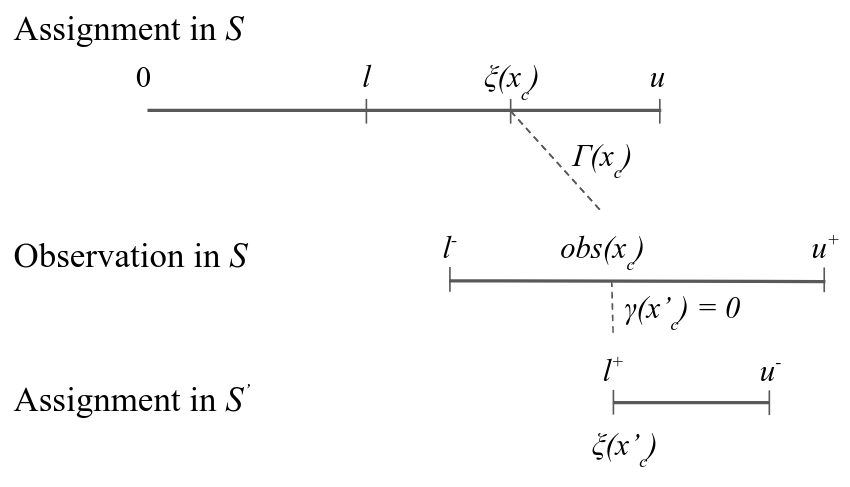
\includegraphics[width=.9\linewidth]{viz-eqn-obs-assign.png}
\caption{\label{fig:obs-assign}We visualize the relationship between realized assignments across \(S\) and \(S'\). In this example, each horizontal line is a timeline monotonically increasing from left to right. Dashed lines represent observation delays. We see how an assignment in \(S\), \assign(x\textsubscript{c})\$, realized observation delay, \(g(x_{c})\), and an observation in \(S\), \(\obs(x_{c})\), lead to an assignment in \(S'\), \assign(x'\textsubscript{c})\$.}
\end{figure}

Note that we receive \(\obs(x_{c})\) from Nature, but make the assignment \(\xi(x'_{c})\) in the
dispatchable form of \(S'\). To be clear, while \(\assign(x_{c})\) is an interval, \((\mathbb{R} \cup
\infty) \times (\mathbb{R} \cup \infty)\), \(\assign(x'_{c})\) is in \(\mathbb{R}\). For a fixed
interval, e.g. \(\obs(x_{c}) \in [t, t]\), we sometimes employ an equivalent representation,
\(\assign(x_{c}) = t\).


Additionally, we sometimes apply \(-\) and \(+\) superscripts to \(l\) and \(u\) to denote the earliest and
latest times respectively that an assignment at those bounds could be observed. For instance, the
relationship in Definition \ref{defn:vdc-obs} simplifies to,

\begin{align}
\label{eqn:obs-assign}
\label{eqn:obs-assign}
\obs(x_{c}) &= [l + \gammabar^-(x_{c}), u + \gammabar^+(x_{c})] \\
\obs(x_{c}) &= [l^-(x_{c}), u^+(x_{c})]
\end{align}

Lastly, we need a means to compare observation spaces if we are to transform variable-delay to
fixed-delay STNUs.

\begin{defn}
\textbf{Observation Space Mapping}

Let \(\mu\) be a mapping from an assignment to a situation, \(\mu : \xi \rightarrow \omega\). To say
that \(\mu(x'_{c}) \subseteq \omega_{v}(x_{c})\) means that, for any assignment of \(x'_{c}\) in \(S'\),
there is an equivalent situation in \(S\) for \(x_{c}\).
\end{defn}

For the transitions below, it is a \emph{valid observation space mapping}, if we can show that
\(\mu(x'_{c}) \subseteq \omega_{v}(x_{c})\). If so, it is guaranteed that any assignment in the
observation space of \(x'_{c}\) also has a valid assignment in the observation space of \(x_{c}\).

We now have the necessary vocabulary and notation to step through the transformations from \(S\) to
\(S'\). These lemmas were first presented in (Bhargava, Nikhil and Muise, Christian and Williams, Brian C., 2018).

\begin{defn}
\textbf{Variable-Delay to Fixed-Delay Transformations}

The \emph{variable-delay to fixed-delay transformations} define a set of observation space mappings,
where there are valid observation space mappings for all the contingent constraints in \(S'\) to \(S\).
\end{defn}

Thus, if there is a satisfying \(\mathcal{S}\) for the fixed-delay observation space of \(S'\), it is guaranteed to
simultaneously satisfy any situation in the variable-delay observation space, \(\Omega_{v}\), of \(S\).

\begin{lemma}
\label{lemma:emulating-fixed}
For any contingent event \(x_c \in X_c\) in \(S\), if \(\gammabar^-(x_c) = \gammabar^+(x_c)\), we emulate
\(\gammabar(x_c)\) in \(S'\) using \(\gamma(x'_c) = \gammabar^+(x_c)\).
\end{lemma}

\begin{proof}
We translate an already fixed-bounded observation delay in the form of \(\gammabar(x_{c})\) to the
equivalent fixed-delay function, \(\gamma(x'_{c})\), thus \(\omega_{f}(x'_{c}) = \omega_{v}(x_{c})\).
\end{proof}

\begin{lemma}
\label{lemma:partially-unobservable}
For any contingent event \(x_c \in X_c\), \(\gammabar^+(x_c) = \infty\), we emulate \(\gammabar(x_c)\) in
\(S'\) as \(\gamma(x'_c) = \infty\).
\end{lemma}

\begin{proof}
There are projections where we would not receive information about \(x_{c}\), therefore we have to act
as if we \emph{never} receive an observation of \(x_{c}\). Any \(\mathcal{S}\) that works when we do not
receive information about \(x_{c}\) would also work when do receive an observation if we choose to
ignore the observation.

None of our decisions depend on \(\xi(x'_{c})\), thus no observation space mapping to \(S\) is
necessary.
\end{proof}

\begin{lemma}
\label{lemma:not-enough-information}
If \(u - l \leq \gammabar^+(x_c) - \gammabar^-(x_c)\), we emulate \(\gammabar(x_c)\) in \(S'\) using
\(\gamma(x'_c) = \infty\).
\end{lemma}

\begin{proof}
We can ignore observations of \(x_{c}\) because they are not guaranteed to narrow where \(\assign(x_c)\)
was assigned in the range \([l, u]\).

Let \(\alpha\) be the range of \(\obs(x_{c})\) when \(\assign(x_{c}) \in [l, l]\). Let \(\beta\) be the
range of \(\obs(x_{c})\) when \(\assign(x_{c}) \in [u, u]\). By Equation \ref{eqn:obs-assign},

\begin{align*}
\alpha &= [l^-(x_{c}), l^+(x_{c})] \\
\beta &= [u^-(x_{c}), u^+(x_{c})]
\end{align*}

We can show that \(u^-(x_{c}) \leq l^+(x_{c})\).

\begin{align*}
u - l &\leq \gammabar^+(x_c) - \gammabar^-(x_{c}) \\
u + \gammabar^-(x_{c}) &\leq l + \gammabar^+(x_{c}) \\
u^-(x_{c}) &\leq l^+(x_{c})
\end{align*}

The lower bound of \(\beta\) is less than the upper bound of \(\alpha\), thus \(\alpha \cap \beta\). An
observation \(\obs(x_{c}) \in [u^-(x_{c}), l^+(x_{c})]\) could be the result of \(\assign(x_{c}) = [l,
l]\), \(\assign(x_{c}) = [u, u]\), or any value \(\assign(x_{c}) \in [l, u]\). Observations provide no
information about the underlying contingent constraint, therefore we ignore \(\obs(x_{c})\).

None of our decisions depend on \(\xi(x'_{c})\), thus no observation space mapping to \(S\) is
necessary.
\end{proof}

\begin{lemma}
\label{lemma:main-tightening}
If \(u - l \geq \gammabar^+(x_c) - \gammabar^-(x_c)\), we can emulate \(\gammabar(x_c)\) under minimal
information by replacing the bounds of \(x_c\) with \(x'_{c} \in [l^+(x_{c}), u^-(x_{c})]\) and letting
\(\gamma(x'_c) = 0\).
\end{lemma}

\begin{proof}
Under Lemma \ref{lemma:main-tightening}, observations \(\obs(x_{c})\) are guaranteed to narrow the range of
\assign(x\textsubscript{c})\$.

We have the same ranges for \(\alpha\) and \(\beta\) as in Lemma \ref{lemma:not-enough-information}, however
we can show that \(u^-(x_{c}) \geq l^+(x_{c})\) instead.

\begin{align*}
u - l &\geq \gammabar^+(x_c) - \gammabar^-(x_{c}) \\
u + \gammabar^-(x_{c}) &\geq l + \gammabar^+(x_{c}) \\
u^-(x_{c}) &\geq l^+(x_{c})
\end{align*}

Thus, receiving an observation is guaranteed to narrow the derived range of \(\assign(x_{c})\). The
transformation tightens the range of \(x'_{c}\) to one where there is maximum ambiguity of the
assignment of \(x_{c}\) while guaranteeing an execution strategy for any assignment of \(x_{c} \in [l,
u]\).

Based on the derivations above, it is clear that \(\mu(x'_{c})\) maps to the observation space where
there is ambiguity as to the projection of \(\assign(x_{c}) \in [l, u]\). We must also show that
\(\mu(x'_{c})\) has mappings to the extrema of \(\xi(x_{c})\). We start with the earliest
\(\assign(x'_{c})\).

$$
\assign(x'_{c}) = l^+(x_{c}) = l + \gammabar^+(x_{c})
$$

We show that that this assignment of \(\xi(x'_{c})\) can be modeled as the following observation in
\(S\).

\begin{align*}
\obs(x_{c}) &\in [l + \gammabar^-(x_{c}), l + \gammabar^+(x_{c})] \\
\obs(x_{c}) &\in [l, l] + \Gamma(x_{c})
\end{align*}

It is possible that \(\xi(x_{c}) = [l, l]\). As such, all observations in \(\obs(x_{c})\) may share the
same execution strategy because the underlying temporal constraints depend on \(\xi(x_{c})\), not
\(\obs(x'_{c})\) or \(\Gamma(x_{c})\). We may expand the range of the observation space when we map to
\(S\) with \(\mu(x'_{c})\).

\begin{align*}
\mu &: l^+(x_{c}) \rightarrow \omega_{v}(x_{c}) \\
\omega_{v}(x_{c}) &= [l + \gammabar^{-}(x_{c}), l + \gammabar^+(x_{c})]
\end{align*}

We see that \(\mu\) has a valid observation space mapping to the minimum of the range of
\(\omega_{v}(x_{c})\). We use the same argument for the maximum.

$$
\assign(x'_{c}) = u + \gammabar^-(x_{c})
$$

Observations anywhere in \([u + \gammabar^-(x_{c}), u + \gammabar^+(x_{c})]\) may share execution
strategies because, it is possible that in all cases, \(\xi(x_{c}) = [u, u]\). We may then expand the
range of the observation space when we map to \(S\).

\begin{align*}
\mu &: u^-(x_{c}) \rightarrow \omega_{v}(x_{c}) \\
\omega_{v}(x_{c}) &= [u + \gammabar^{-}(x_{c}), u + \gammabar^+(x_{c})]
\end{align*}

Thus, \(\mu(x'_{c})\) maps to the maximum of the range of \(\omega_{v}(x_{c})\). The transition creates
assignments in \(S'\) that map to the entire \(\omega_{v}(x_{c})\) in \(S\).

\end{proof}

This concludes the modifications required to transform a contingent event \(x_{c} \in X_{c}\) in \(S\)
to its equivalent \(x'_{c} \in X_{c}\) in \(S'\). What remains is to address the transformation of
requirement links, \(x_{r} \in X_{r}\), in \(S\) such that their transformed equivalents, \(x'_{r} \in
X_{r}\) in \(S'\), express the same execution semantics in \(S'\) as they did in \(S\). We will demonstrate
the correctness of the transformations after Lemma \ref{lemma:applied-execution}.

\begin{lemma}
\label{lemma:execution}
If we have contingent link \(\conedge{X}{C}{}\) with duration \([l, u]\), outgoing requirement link
\(\edge{C}{Z}{}\) with duration \([u, v]\) with an unobservable \(C\), and contingent link
\(\conedge{C}{Y}{}\) with range \([\gammabar^-(x_{c}), \gammabar^+(x_{c})]\), we can emulate the role of
the original requirement link during execution with a new link \(\edge{Y}{Z}{}\) with bounds \([u -
max(\gammabar^-(x_{c}), XY - u), v - min(\gammabar^+(x_{c}), XY - l)]\), where \(XY\) is the true
duration of \(\conedge{X}{Y}{}\).
\end{lemma}

\begin{proof}
See Figure \ref{fig:combined-figure}c for reference. From an execution perspective, \(X\) and \(Y\) are
the only events that can give us any information that we can use to reason about when to execute \(Z\)
(since \(C\) is wholly unobservable).

If we execute \(Z\) based on what we learn from \(Y\), then we use our information from \(Y\) to make
inferences about the true durations of \(\conedge{X}{C}{}\) and \(\conedge{C}{Y}{}\) based on
\(\conedge{X}{Y}{}\). We know that the lower-bound of \(\conedge{C}{Y}{}\) is at least \(XY - b\) and that
its upper-bound is at most \(XY - a\). But we also have the a priori bounds on the contingent link
that limit its range to \([\gammabar^-, \gammabar^+]\). Taken together, during execution we can infer
that the true bounds of \(\conedge{C}{Y}{}\) are \([max(\gammabar^-, XY - b), min(\gammabar^+, XY -
a)]\). Since we have bounds only on \(Z\)'s execution in relation to \(C\), we can then infer a
requirement link \(\edge{Y}{Z}{}\) with bounds \([u - max(\gammabar^-, XY - b), v - min(\gammabar^-,
XY - a)]\).

If we try to execute \(Z\) based on information we have about \(X\), we must be robust to any possible
value assigned to \(\conedge{X}{C}{}\). This means that we would be forced to draw a requirement link
\(\edge{X}{Z}{}\) with bounds \([u+b, v+a]\). But we know that \(u - max(\gammabar^-, XY - b) \leq u +
b - XY\) and \(v - min(\gammabar^-, XY - a) \geq v + a - XY\), which means that the bounds we derived
from \(Y\) are at least as expressive as the bounds that we would derive from \(X\).
\end{proof}

Since we have a local execution strategy that depends on the real value of \(XY\), we can try to apply
this strategy to the contingent link that we restricted in Lemma \ref{lemma:main-tightening}, in
order to repair the remaining requirement links.

\begin{lemma}
\label{lemma:applied-execution}
If we have an outgoing requirement link \(\edge{C}{Z}{}\) with duration \([u, v]\), where \(C\) is a
contingent event, we can emulate the role of the original requirement link by replacing its bounds
with \([u - \gammabar^-(x_{c}), v - \gammabar^+(x_{c})]\).
\end{lemma}

\begin{proof}
See Figure \ref{fig:combined-figure}d for reference. If we directly apply the transformation from
Lemma \ref{lemma:execution} and Figure \ref{fig:combined-figure}c to our original STNU, we introduce
complexity through the need to reason over \(min\) and \(max\) operations in our link bounds. However,
from Lemma \ref{lemma:main-tightening}, we know that in a controllability evaluation context, it is
acceptable for us to simplify the \(\conedge{X}{Y}{}\) link to a stricter range of \([a + \gammabar^+,
b + \gammabar^-]\), instead of \([a + \gammabar^-, b + \gammabar^+]\). This means that for the purpose
of evaluating controllability, we can assume \(a + \gammabar^+ \leq XY \leq b + \gammabar^-\). When we
evaluate the requirement link \(\edge{Y}{Z}{}\), we see \(max(\gammabar^-, XY - b) = \gammabar^-\) and
\(min(\gammabar^+, XY - a) = \gammabar^+\). This gives us bounds of \([u - \gammabar^-, v -
\gammabar^+]\) for the \(\edge{Y}{Z}{}\) requirement link as seen in Figure \ref{fig:combined-figure}d.
\end{proof}

Lemma \ref{lemma:applied-execution} handles outgoing requirement edges connected to contingent
events. In addition, we must handle incoming edges.

\begin{corollary}
\label{corollary:reversed}
If we have an incoming requirement link \(\edge{Z}{C}{}\) with duration \([u, v]\), where \(C\) is a
contingent event, we can replace the bounds of the original requirement link with \([u +
\gammabar^+(x_{c}), v + \gammabar^-(x_{c})]\).
\end{corollary}

\begin{proof}
A requirement link \(\edge{Z}{C}{}\) with bounds \([u, v]\) can be immediately rewritten as its reverse
\(\edge{C}{Z}{}\) with bounds \([-v, -u]\). After reversing the edge, we can apply Lemma
\ref{lemma:applied-execution} to get \(\edge{Y}{Z}{}\) with bounds \([-v - \gammabar^-, -u -
\gammabar^+]\), which we can reverse again to get \(\edge{Z}{Y}{}\) with bounds \([u + \gammabar^+, v +
\gammabar^-]\).
\end{proof}

After applying Lemma \ref{lemma:main-tightening}, despite the limited expected range of assignments in
\(x'_{c}\) in \(S'\) compared to \(x_{c}\) in \(S\), we can show that Lemma \ref{lemma:applied-execution}
guarantees a satisfying schedule for any \(\obs(x_{c}) \in [l^-(x_{c}), u^+(x_{c})]\) using an
\(\mathcal{S}\) that employs \emph{buffering} and \emph{imagining} contingent events.

\begin{defn}
\textbf{Buffering}

\emph{Buffering} a contingent event \(x_{c}\) is an execution strategy where, if \(x_{c}\) is observed
earlier than the lower bound of the observation space \(\obs(x_{c}) < \omega_{f}^-(x'_{c})\), we
assign \(\xi(x'_{c})\) to the lower bound of the observation space, \(\xi(x'_{c}) =
\omega_{f}^-(x'_{c})\).
\end{defn}

\begin{defn}
\textbf{Imagining}

\emph{Imagining} a contingent event \(x_{c}\) is an execution strategy where, if \(x_{c}\) is observed later
than the upper bound of the observation space, \(\obs(x_{c}) > \omega_{f}^+(x'_{c})\), we assign
\(\xi(x'_{c})\) to the upper bound of the observation space, \(\xi(x'_{c}) = \omega_{f}^+(x'_{c})\).
\end{defn}

\begin{lemma}
If \(S'\) is fixed-delay controllable after applying Lemmas \ref{lemma:main-tightening}, \ref{lemma:execution},
and \ref{lemma:applied-execution} to contingent event \(Y\) with following requirement event \(Z\), there is a
valid \(\mathcal{S}\) for any observation in the observation space of \(S\), \(\omega_{v}(Y) = [a^-(Y),
b^+(Y)]\).
\end{lemma}

\begin{proof}
We first note the observation space of \(S'\) is a subinterval of the original observation space of
\(S\), \(\omega_{f}(Y') \subset \omega_{v}(Y)\), and there are two distinct ranges of observations that
are not in \(\omega_{f}(Y')\).

\begin{align*}
\omega_{f}(Y') &= [a + \gammabar^+(Y), b + \gammabar^-(Y)];~\omega_{v}(Y) = [a + \gammabar^-(Y), b + \gammabar^+(Y)] \\
\omega_{f}(Y') &\not\supset [a + \gammabar^-(Y), a + \gammabar^+(Y))~~(\textit{"Early" observations}) \\
\omega_{f}(Y') &\not\supset (b + \gammabar^+(Y), b + \gammabar^+(Y)]~~(\textit{"Late" observations})
\end{align*}

We address the early observations first. The range of early assignments of \(\xi(Y)\) in \(S\) that we
care about are the ones that could produce an observation \(\obs(Y) \leq a + \gammabar^+(Y)\), which
is \(\xi(Y) = [a, a + (\gammabar^+(Y) - \gammabar^-(Y))]\). We rewrite the range of early assignments
as \(\xi(Y) = a + (\gammabar^+(Y) - \gammabar^-(Y)) - \epsilon\), where \(0 \leq \epsilon \leq
(\gammabar^+(Y) - \gammabar^-(Y))\). By the semantics of \(S\), the range of assignments of \(\xi(Z)\) is
then,

\begin{align*}
\xi(Z) &= [a + (\gammabar^+(Y) - \gammabar^-(Y)) - \epsilon, a + (\gammabar^+(Y) - \gammabar^-(Y)) - \epsilon] + [u, v] \\
\xi(Z) &= [a + u + (\gammabar^+(Y) - \gammabar^-(Y)) - \epsilon, a + v + (\gammabar^+(Y) - \gammabar^-(Y)) - \epsilon]
\end{align*}

The earliest assignment of \(Y'\) in \(S'\) is \(\xi(Y') = a + \gammabar^+(Y)\). By the semantics of \(S'\),
the range of assignments of \(\xi(Z')\) is then,

\begin{align*}
\xi(Z') &= [a + \gammabar^+(Y), a + \gammabar^+(Y)] + [u - \gammabar^-(Y), v - \gammabar^+(Y)] \\
\xi(Z') &= [a + u + (\gammabar^+(Y) - \gammabar^-(Y)), a + v]
\end{align*}

We see that \(\xi(Z') \subseteq \xi(Z)\) for any \(\epsilon\), meaning the execution strategy when
\(\xi(Y') = a + \gammabar^+(Y)\) results in a valid assignment of \(\xi(Z)\) for all early observations
of \(\xi(Y)\). We are safe to buffer early observations to \(\xi(Y') = a + \gammabar^+(Y)\).

We use the same argument for imagining late observations. The range of late assignments of \(\xi(Y)\)
in \(S\) that we care about are the ones that could produce an observation \(\obs(Y) \geq b +
\gammabar^-(Y)\), which is \(\xi(Y) = b - (\gammabar^+(Y) - \gammabar^-(Y)) + \epsilon\). By the
semantics of \(S\), the range of assignments of \(\xi(Z)\) is then,

\begin{align*}
\xi(Z) &= [b - (\gammabar^+(Y) - \gammabar^-(Y)) + \epsilon, b - (\gammabar^+(Y) - \gammabar^-(Y)) + \epsilon] + [u, v] \\
\xi(Z) &= [b + u - (\gammabar^+(Y) - \gammabar^-(Y)) + \epsilon, b + v - (\gammabar^+(Y) - \gammabar^-(Y)) + \epsilon]
\end{align*}

The last assignment of \(Y'\) in \(S'\) is \(\xi(Y') = b + \gammabar^-(Y)\). By the semantics of \(S'\),
the range of assignments of \(\xi(Z')\) is then,

\begin{align*}
\xi(Z') &= [b + \gammabar^-(Y), b + \gammabar^+(Y)] + [u - \gammabar^-(Y), v - \gammabar^+(Y)] \\
\xi(Z') &= [b + u, b + v - (\gammabar^+(Y) - \gammabar^-(Y))]
\end{align*}

We see that \(\xi(Z') \subseteq \xi(Z)\) for any \(\epsilon\), meaning the execution strategy when
\(\xi(Y') = b + \gammabar^-(Y)\) results in a valid assignment of \(\xi(Z)\) for all late observations
of \(\xi(Y)\). In practice, there is no reason to wait until after \(\obs(Y) = b + \gammabar^-(Y)\) to
receive a late observation. As soon as we see the clock has reached \(b + \gammabar^-(Y)\), we are
safe to imagine that \(\obs(Y)\) has been received.
\end{proof}

We can examine a concrete example of Lemmas \ref{lemma:main-tightening}, \ref{lemma:execution}, and
\ref{lemma:applied-execution} to show equivalence in the transformation from Figure
\ref{fig:combined-figure}a to \ref{fig:combined-figure}d. We start by building an example of
\ref{fig:combined-figure}a. Let \(\conedge{X}{C}{[2, 5]}\) with \(\gammabar(C) \in [1, 2]\) and
\(\edge{C}{Z}{[11, 20]}\). If we learn of event \(C\) at time 4, then one possibility is that the
realized duration of \(C\) could have been 2 with an observation delay of 2. In this case, event \(Z\)
must be executed in \([13, 22]\). However, if the realized duration of \(C\) were 3 with an observation
delay of 1, then \(Z\) would fall in \([14, 23]\). Given we cannot distinguish between the
possibilities, we take the intersection of the intervals, yielding \(Z \in [14, 22]\). Likewise, if we
learn of \(C\) at time 6, then \(C\) could have been realized at time 5 with an observation delay of 1
or it could have been realized at time 4 with an observation delay of 2. In the first case, \(Z\) must
then fall in \([16, 25]\), while in the second, \(Z\) would fall in \([15, 24]\). The intersection yields
\([16, 24]\).

By the semantics represented in Figure \ref{fig:combined-figure}d, we can build an equivalent
network with \(\gamma(Y) = 0\) by setting \(\conedge{X}{Y}{[4, 6]}\) and \(\edge{Y}{Z}{[10, 18]}\). If \(Y\)
is observed at time 4, \(Z\) must be executed in \([14, 22]\). If \(Y\) is observed at time 6, \(Z\) then
must be executed in \([16, 24]\). The execution semantics for both cases match the equivalent networks
from \ref{fig:combined-figure}a described above.

\subsection{Dynamic Scheduling through Real-Time Execution Decisions}
\label{sec:orgd757cee}
\label{sec:dynamic-scheduling}

An STNU, \(S\), that exhibits dynamic controllability can be \emph{scheduled} dynamically (or \emph{online}). At
a high-level, dynamic scheduling is the process of mapping the history of event assignments to the
execution time of future free events. We follow the scheduling work by Hunsberger
(Hunsberger, Luke, 2013, Hunsberger, Luke, 2016), which describes an \(O(N^{3})\) procedure, FAST-EX, for
dynamic scheduling of STNUs. At its core is the notion of \emph{Real-Time Execution Decisions} (RTEDs),
which map a timepoint to a set of requirement events to be executed and are generated based on
\emph{partial schedules} of STNUs being executed. \texttt{WAIT} decisions may also be produced, reflecting the
need to wait for the assignment of a contingent event before continuing. RTED-based scheduling
applies a dynamic programming paradigm by first creating a dispatchable form of temporal constraints
offline, updating the dispatchable form as the partial schedule is updated online, and querying the
dispatchable form online to quickly find the next free event to schedule (Hunsberger, Luke, 2009).

\begin{defn}
\textbf{Real-Time Execution Decisions} (Hunsberger, Luke, 2009)

A \emph{Real-Time Execution Decision} is a two-tuple \(\langle t, \chi \rangle\), where:
\begin{itemize}
\item \(t\) is a time with domain \(\mathbb{R}\),
\item \(\chi\) is a set of \(x_{r} \in X_{r}\) to be executed at time \(t\)
\end{itemize}
\end{defn}

\begin{defn}
\textbf{Partial Schedule}

A \emph{Partial Schedule} for an STNU is a mapping \(\xi ~:~ t \rightarrow \mathbb{R}\), where \(t\) is a
proper subset of timepoints in \(X\) with domain \(\mathbb{R}\).
\end{defn}

A partial schedule is the set of assignments \emph{so far} during execution. They can be represented by
\(\xi_{t} = \{ (A, \xi(A) \}\) notation, meaning that by some time \(t\), event \(A\) has been scheduled
at time \(\xi(A)\). By definition, all STNU executions begin with a partial schedule \(\xi_{0} =
\emptyset\), meaning no timepoints have been assigned at time \(0\). As timepoints are executed, the
partial schedule grows. For example, if event \(A\) is assigned to \(1\) and \(B\) to \(2\), then at time
\$2, \(\xi_{2} = \{ (A, 1), (B, 2) \}\).

The dispatchable form employed by FAST-EX is the \emph{AllMax} distance graph, which is produced by the
Morris \(O(N^{4})\) DC-checking procedure (Morris, Paul, 2006).

\begin{defn}
\textbf{AllMax Distance Graph} (Morris, Paul and Muscettola, Nicola, 2005)

The \emph{AllMax} distance graph is a distance graph exclusively consisting of unlabeled and upper-case
edges.
\end{defn}

The key idea of FAST-EX is maintaining accurate distances from a zero point, \(Z\), of the graph to
all events. At the outset of execution, all events from \(S\) are present as nodes in \emph{AllMax}. As
contingent events are observed, \emph{AllMax} performs update steps using Dijkstra Single Source/Sink
Shortest Path (SSSP) to maintain distances to unexecuted events, while also removing executed
events. We include pseudo-code of the update step in Figure \ref{alg:fast-ex-update}.

\begin{algorithm}
\SetAlgoLined
\SetKwFunction{Return}{return}
\SetKwInput{Input}{Input}
\SetKwInput{Output}{Output}
\SetKwInput{Algorithm}{\textsc{FAST-EX Update}}
\SetKwInput{Initialize}{Initialization}
\SetKwIF{If}{ElseIf}{Else}{if}{then}{else if}{else}{endif}
\Indm
\Input{Time $t$; Set of newly executed events $\texttt{Exec} \subseteq X_{e} \cup X_{r}$; AllMax Graph $G$; Distance matrix $D$, where $D(A, B)$ is the distance from $A$ to $B$}
\Output{Updated $D$}
\Indp
\Algorithm{}
\Indp
\For{each continent event $C \in \texttt{Exec}$} {
    Remove each upper-case edge, $\edge{Y}{A}{C:-w}$, labled by $C$\;
    Replace each edge from $Y$ to $Z$ with the strongest replacement edge\;
}
\For{each event $E \in \texttt{Exec}$} {
    Add lower-bound edge $\edge{E}{Z}{-t}$\;
}
For each event $X$, update $D(X, Z)$ using Dijkstra Single-Sink Shortest Paths\;
\For{each event $E \in \texttt{Exec}$} {
    Add upper-bound edge $\edge{Z}{E}{t}$\;
}
For each event $X$, update $D(Z, X)$ using Dijkstra Single-Source Shortest Paths\;
\caption{Algorithm for updating distances for all events in relation to $Z$ upon the execution of an event. Adapated from \citeprocitem{3}{[3]}, Fig. 19.}
\label{alg:fast-ex-update}
\end{algorithm}

Given an accurate distance matrix, we find the next RTED as follows. Let \(U_{x}\) be the set of
unexecuted free timepoints. If \(U_{x}\) is empty, then the RTED is to \texttt{WAIT}. Otherwise, we find the
lower bound of the earliest executable time point and the set of executable events associated with
it.

\begin{align*}
t &= \min\{-D(X, Z)~|~X \in U_{x}\} \\
\chi &= \{X \in U_{x}~|~-D(X, Z) = t\}
\end{align*}

We cannot execute events in the past. Let \(\texttt{now}\) be the current time, i.e. the last timepoint
captured in \(\xi\). It is possible that \(t \leq \texttt{now}\), in which case we must reassign \(t\) to
guarantee that \(t > \texttt{now}\). To do so, we update \(t\) as follows, where \(t_{U}\) is earliest
\emph{upper} bound of the executable timepoints,

\begin{align*}
t_{U} &= \min\{D(Z, X)~|~X \in U_{x}\} \\
t &= \cfrac{\texttt{now} + t_{U}}{2}
\end{align*}

So long as \(t_{U} > \texttt{now}\), we know that the reassignment of \(t\) ensures \(t > \texttt{now}\).
\end{document}